\documentclass[../dejiny-rodu-prusiku.tex]{subfiles}

\begin{document}

% str 183 @ 211
\chapter{Větev nebřežiny}

Zakladatel Josef Prusík

1796 - 1875

Na řadě je nyní vyprávění o členech našeho rodu, kteří se usadili ve vesnici Nebřežiny u Plas a o jejich potomcích.

Stavitel Martin Prusík v Plasích, který sem přišel v druhé polovině XVIII. století ze Sedlce, měl druhého syna, který byl pokřtěn na jméno Josef. Narodil se 20. 3. 1796 v Plasích. Nevyučil se však u otce zednickému řemeslu, ale stal se obuvníkem. V blízké, romanticky položené vesničce na Střele, Nebřežinech měl obuvnickou živnost Říha. Měl tam domek na pravém břehu Střely a sem se přiženil v roce 1816 Josef Prusík. V té době zde také bydlel již jeho bratr František, který byl zedníkem. Manželkou Josefa stala se Jana Říhová, narozená 24. 5. 1795 v Nebřežinech. Měli spolu deset dětí, ale jen šest jich dospělo. Byly to dcery Josefa, Marie a Alžběta a synové František, Josef a Emanuel.

Když byl založen v roce 1144 klášter v Plasích, dal mu kníže Vladislav II. kromě jiných vsí také Nebřežiny. Ve XIII. století založil klášter poplužní dvůr a opat Gottfried vysadil roku 1412 ves Nebřežiny právem zákupním. Přes Nebřežiny vedla odedávna zemská stezka, která spojovala celý sever s Plzní. Proto klášter zřídil tu již v dávné době most přes řeku Střelu. Od roku 1601 vybíra­lo se v Nebřežinech clo na mostě a klášteru vynášelo hodné peněz, neboť za obchodem přes most jezdilo mnoho lidí. Za císaře Rudolfa II. každý, kdo jel po mostě s těžkým vozem nebo se saněmi platil český groš, z vozu lehčího po sedmi malých penězích, z každého koně zapřáhnu­tého nebo nezapřáhnutého po dvou bílých penězích, z vo­lů a krav po třech penězích, ze tří telat, koz a vepřů po dvou penězích a z menšího dobytka po jednom penězi. I každý pěší, jda přes most, musel dát jeden peníz. Za třicetileté války hrnuly se tady často vojenské tlupy a tehdy také byla ves docela spálena. Po této zhoubné vál­ce, živořili zde jen dva osadníci. V této obci narodil se v roce 1820 Václav Levý, pozdější slavný sochař čes­ký, předchůdce Myslbekův. Členové našeho rodu znali se tedy s ním od dětství.

Své výrobky prodával Josef Prusík nejen ve vsi, ale i po širokém okolí, zvláště také do Plas. Tam žil jeho bratr Antonín.

Nejstarším dítětem Josefa Prusíka byla dcera Josefa. Narodila se 19. 12. 1820 a v roce 1844 se vdala za Josefa Kříže, dělníka v parketárně v Nebřežinech. Měli asi šest dětí a nejméně deseti let dospěly tři. Josef narozený v roce 1846, František 1851 a dcera Jana 1853. Josefovi byl
% str 184 @ 212
vydán, podle našeho pátrání křestní list v roce 1872. Bylo to asi za účelem jeho sňatku. Ještě před zhoubnou povodní odstěhovala se rodina Josefy Křížové roz. Prusíkové z Nebřežin a přes nejusilovnější snahu nepodaři­lo se najiti místo jejich dalšího pobytu. Je však pravdě­podobné, že někde žijí v dalších generacích její potom­ci.

Ještě před Josefou, abychom byli přesní, narodila se dcera Marie, která se v roce 1840 provdala za Josefa Žaloudka, mlynářského pomocníka a později krupaře v Nebřežinech. Marie Prusíková narodila se 21. 11. 1818. Měla pět dětí, ale celá její rodina zahynula při kata­strofální povodni v roce 1872. Bylo to 25. května. S ní také zahynula její sestra Alžběta, která bydlela v jiném stavení v Nebřežinech a to se svým otcem Josefem Prusíkem, který byl již vdovcem. Jeho manželka Jana roz. Říhová zemřela rok před povodní 13. 4. 1871.

Povodeň z května roku 1872 byla opravdovou katastrofou nejen v Nebřežinech ale do značné míry i v povodí Be­rounky a v Praze. Jak to tehdy bylo?

\section{O povodni v Nebřežinech}
Dne 25. května 1872 přišla velká průtrž mračen na celý plasský kraj. Nejhůře bylo na Potvorovské hoře, kde se sesula celá stráň i s částí postavené dráhy a tehdy se také utvořilo jezírko, na jehož dně leží pohřbeny kolej­nice nové dráhy. Byla to nově stavěná dráha z Plzně do Duchcova a mezi stanicí Mladotice a Přehořovem můžete vidět toto tiché jezírko se zádumčivými lesy kolem, které je svědkem katastrofy. V mladotickém rybníku, po němž dnes již není stopy od těch dob, nahromadilo se tolik vo­dy, že se jeho hráz protrhla a voda se řítila na Plasy.

Pod hrází tohoto rybníka byl mlýn. Je zajímavé, že obydlí bylo ušetřeno, jen některé budovy byly zničeny. Vyprá­ví se, že na dvůr mlynářův připlaveno bylo množství věcí, postele, židle, almary, stoly a v jedné almaře, že bylo nalezeno 4000.- zlatých.

Voda brala s sebou vše, co jí bylo v cestě. Na pile v Pla­sích vzala zásoby prken a špalků, dále strhla most přes Střelu a dva domky. To všechno zatarasilo rychlý spád a volný odtok řeky, která ústí do tak zvaných hor k Nebřežinám. Za chvíli bylo přízemí konventu pod vodou a tam se utopil důchodní Siebert a jedna žena.

Hroznější důsledky však měla velká voda v Nebřežinech. Přišla tam až v noci a odnesla osm domků i s obyvateli, mlýn, strhla most a připlavila dva domky a stodůlku z Plas. v té době bydleli v Nebřežinech dělníci, kteří pra­covali na stavbě nové dráhy. Těch se utopilo osmnáct. Ostatních obyvatel Nebřežin se utopilo padesát, celkem bylo tedy obětí šedesát osm lidí.

% str 185 @ 213
Jak rychle tehdy voda stoupala, bylo vidět z pozorování u staroměstských mlýnů v Praze. Dne 25. května odpoledne v pět hodin byl stav vody pět a půl palce nad normálem. V jednu hodinu v noci bylo to již pa­desát palců nad normálem a 26. května ve dvě hodiny odpoledne dokonce 2 sáhy, to je hodně pře 100 pal­ců.

Neštěstí toto značné postihlo náš rod. Utopila se Ma­rie Žaloudková roz. Prusíková s celou rodinou a o zká­ze jejich domku je psáno v tehdejším „Světozoru“, vydá­vaném Dr. Skrejšovským, toto: "Hrůza nás obešla, když jsme spatřili, jak se domek plovoucí počíná ztrácet, byl vlnami a plovoucími kládami roztříštěn. Jen jeden muž trámu se drže, asi za půldruhé hodiny živ na břeh byl vyvržen. Manželka Žaloudkova byla nalezena mrtvá pod Nebřežinami, držíc se jednou rukou lesního stromu, o který se byla ve smrtelném zápase zachytila a v druhé ruce své dítě." Alžběta Prusíková narozená 7. 7. 1829 v Nebřežinech zůstala svobodná a když přišla ta zkáza na Nebřežiny v roce 1872 ošetřovala svého starého otce. Byl by také málem zahynul, byl již po pás ve vodě, ale jeho dce­ra vynesla ho ještě z chalupy. Pak se do chalupy ještě vrátila pro peřiny, vtom voda chalupu pozdvihla a za­točila a víckrát již nikdo Alžbětu Prusíkovou nespatřil. Tak zahynuly dvě dcery Josefa Prusíka v roce 1872 a děti jedné z nich, provdané Žaloudkové.

Josef Prusík, obuvník v Nebřežinech zemřel za necelé tři roky po tom, dne 9. ledna 1875. Dožil se 79 let.

Prvním synem Josefa Prusíka, který dospěl, byl František. Narodil se v Nebřežinech 18. 1. 1823. Vyučil se u otce ševcovině a pustil se pak do světa. Pracoval jako to­varyš v Plzni, Praze, v roce 1840 šel vandrem do Vídně a pak až do Štyrska, Korutan, Tyrol, kde navštívil i Brixen, kde byl vězněn Karel Havlíček Borovský. František Prusík vandroval pak přes Meran, Trident do Voralberku a tam pracoval ve Feldkirchu. Pak přešel hra­nice do Švýcar, podíval se i do Kostnice, kde byl upálen Mistr Jan Hus. Ve Švýcarsku pracoval celé čtyři roky, tam se však píchl do ruky šídlem, ale tehdy nebylo ještě postaráno o nemocného, když byl práce neschopen. Proto se vrátil v roce 1846 domů a 12. října 1847 se po prvé oženil. Usadil se v Plasích a vzal si za ženu dceru kostelníka Marii Bradáčovou, nar. 16. 7. 1826. Z tohoto manžel­ství měl čtyři děti, tři syny a dcerku, ale všechny zemře­ly v dětství. I první manželka Františka Prusíka Marie, zemřela brzy a to 4. 12. 1855. Za půl roku oženil se Fran­tišek Prusík po druhé. Byla to Marie roz. Beránková z Lednice, narozená 18. 1. 1826. S ní měl František tři dcery, z nichž dvě dospěly, Anna a Marie. Marie Prusíková nar. 10. 5. 1862 v Plasích, provdala se ve dvaceti letech za hokynáře Řeháka v Praze, ale po porodu zemřela již 15. 11. 1882. Také dítě nezůstalo na živu. Druhou dcerou z tohoto
% str 186 @ 214
manželství Františka Prusíka byla Anna a po ní žijí potomci. Narodila se 21. 11. 1857 v Plasích. Provdala se za obuvníka Blažeje Huttera, Němce ve Vroutku. S ním měla několik dětí, z nichž jen dvě dospěly. Anna Hutterová roz. Prusíková zemřela však poměrně mladá 17. 12. 1892. Její potomci jsou již Němci. Dcera Anna narodila se 30. 5. 1881 a byla provdaná Richterová v Ústí nad Labem. Zemřela za světové války 25. 5. 1917 v Zálezlech u Ústí nad Lab. Anna Richterová roz. Hutterová z Vroutku měla dceru a syna. Její dcera Marie narodila se 1. 4. 1910 v Ústí nad Labem a dnes je provdaná Goldaová a je bezdětná. Po odsunu z republiky žije v rá­zovitém městečku Waiblingen u Stuttgartu, Schlesierweg 2. Dříve bydlela v Norimberku. Její bratr Rudolf Richter, narodil se 15. 10. 1912 a žil v městě Geisingen u Kostnice. Byl z druhé světové války těžkým invalidou a zemřel 22. 3. 1967. Má syna Rudolfa Richtera nar. 6. 8. 1940. Ten bydlí ve Stuttgartě, Engelboldstrasse 102. Jeho manžel­kou je Španělka z Valencie. Mají dceru Michaelu nar. 29. 12. 1966.

Druhým dítětem Anny Hutterové roz. Prusíkové byl syn Arnošt. Narodil se 20. 7. 1890, usadil se v Žatci, kde byl úředníkem města. Měl syna a dceru. Podle svědků, Čechů, kteří ho znali, nikdy nevystupoval agresivně proti českému národu, k němuž po matce patřil. Po válce byl odsunut a zemřel v Halle v NDR 7. 6. 1963. Jeho syn Arnošt Hutter vystudoval lékařství v Praze. Narodil se 24. 9. 1914 v Žatci a dnes žije v městě Moosburg v Bavorsku, Statzenbachstrasse 1. Má tam pěknou vilu a vlastní ordi­naci. Jeho dcerka Birgit Hutterová je narozena 14. 2. 1959. Druhým dítětem Arnošta Huttera, rodáka z Vroutku je dce­ra Hilda. Narodila se 8. 9. 1924, byla hudebně nadána, ale toto studium ji překazila válka. Dnes je provdaná Lebiodaová a žije v Halle nad Saalou C 2, Vogelherd 25. Má dva syny, Petra nar. 31. 8. 1950 a Haralda Lebiodu nar. 1. 11. 1952.

Druhá manželka Františka Prusíka, obuvníka z Plas, Marie, rozená Beránková zemřela také poměrně mladá 15. 7. 1872. A tak se František oženil po třetí. Dne 14. ledna 1873 oženil se František s Josefou Sillabovou, nar. 26. 2. 1840. Její rodiště bylo Dammerschlag u Tachova. Do manželství s Františkem přivedla si nemanželskou dcerku Annu, nar. 1869 v Černošíně u Stříbra. Ta byla později provdaná Soprová v Dobré Vodě u Českých Budějovic. Měla čtyři syny a jednu dceru Annu, provdanou Komárkovou. Zmiňujeme se o těchto dětech přesto-že pokrevně nepatří k našemu rodu proto, že všichni byli v nejpřátelštějším styku s rodem Prusíků.

František Prusík měl pak s Josefou Sillabovou několik dětí, ale jen dvě dospěly. Jeho čtyřletého synka přejel vůz naložení zemí a byl okamžitě mrtev.
Obuvník František Prusík byl písmákem. Vedl rodinnou kroniku, ale zapisoval v ní i všechny události místní, krajové a zemské. Rok 1868, tedy sto let před tím, co sepisujeme
% str 187 @ 216
sujeme tyto dějiny, popisuje stručné takto: "Dne 30. března 1860 bylo takové krupobití, že padaly kroupy jako vejce, rozbito bylo jak obilí tak stromoví. Na to pak celé léto nepršelo po celé české zemi." A o dalších letech píše František toto: "V roce 1869 bylo zase takové sucho, že lidé hladověli a v roce l870 byla dlouhotrvající zima, takže 25. března napadlo tolik sněhu, že toho nebylo pamětníka." A tak čtenáři těchto dějin uvidí, zda to počasí se bude po sto letech opakovat.

% str 186+1 @ 215
\begin{figure}
\centering
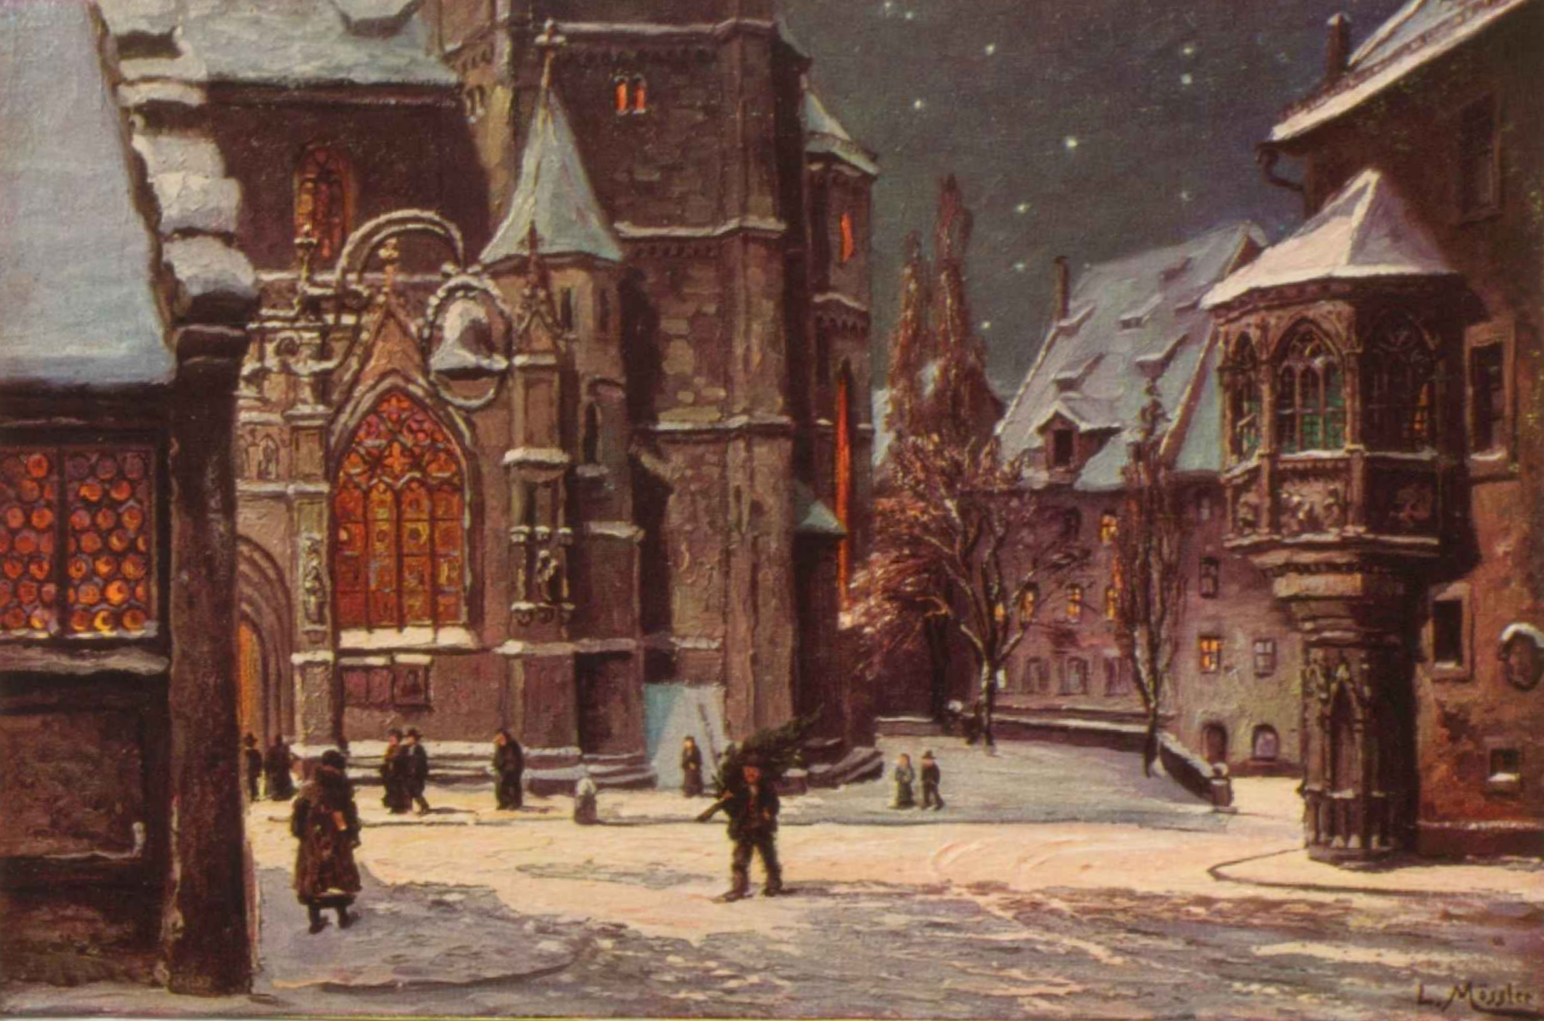
\includegraphics[width=\textwidth, height=\textheight, keepaspectratio]{215-a-norimberk}
\caption{Norimberk, kde pracuje Rudolf Prusík, rodák z Veletic u Žatce. Tomáš Prusík, rodák ze Sedlice, byl jeho pradědem}
\label{fig:215-a-norimberk}
\end{figure}

\begin{figure}
\centering
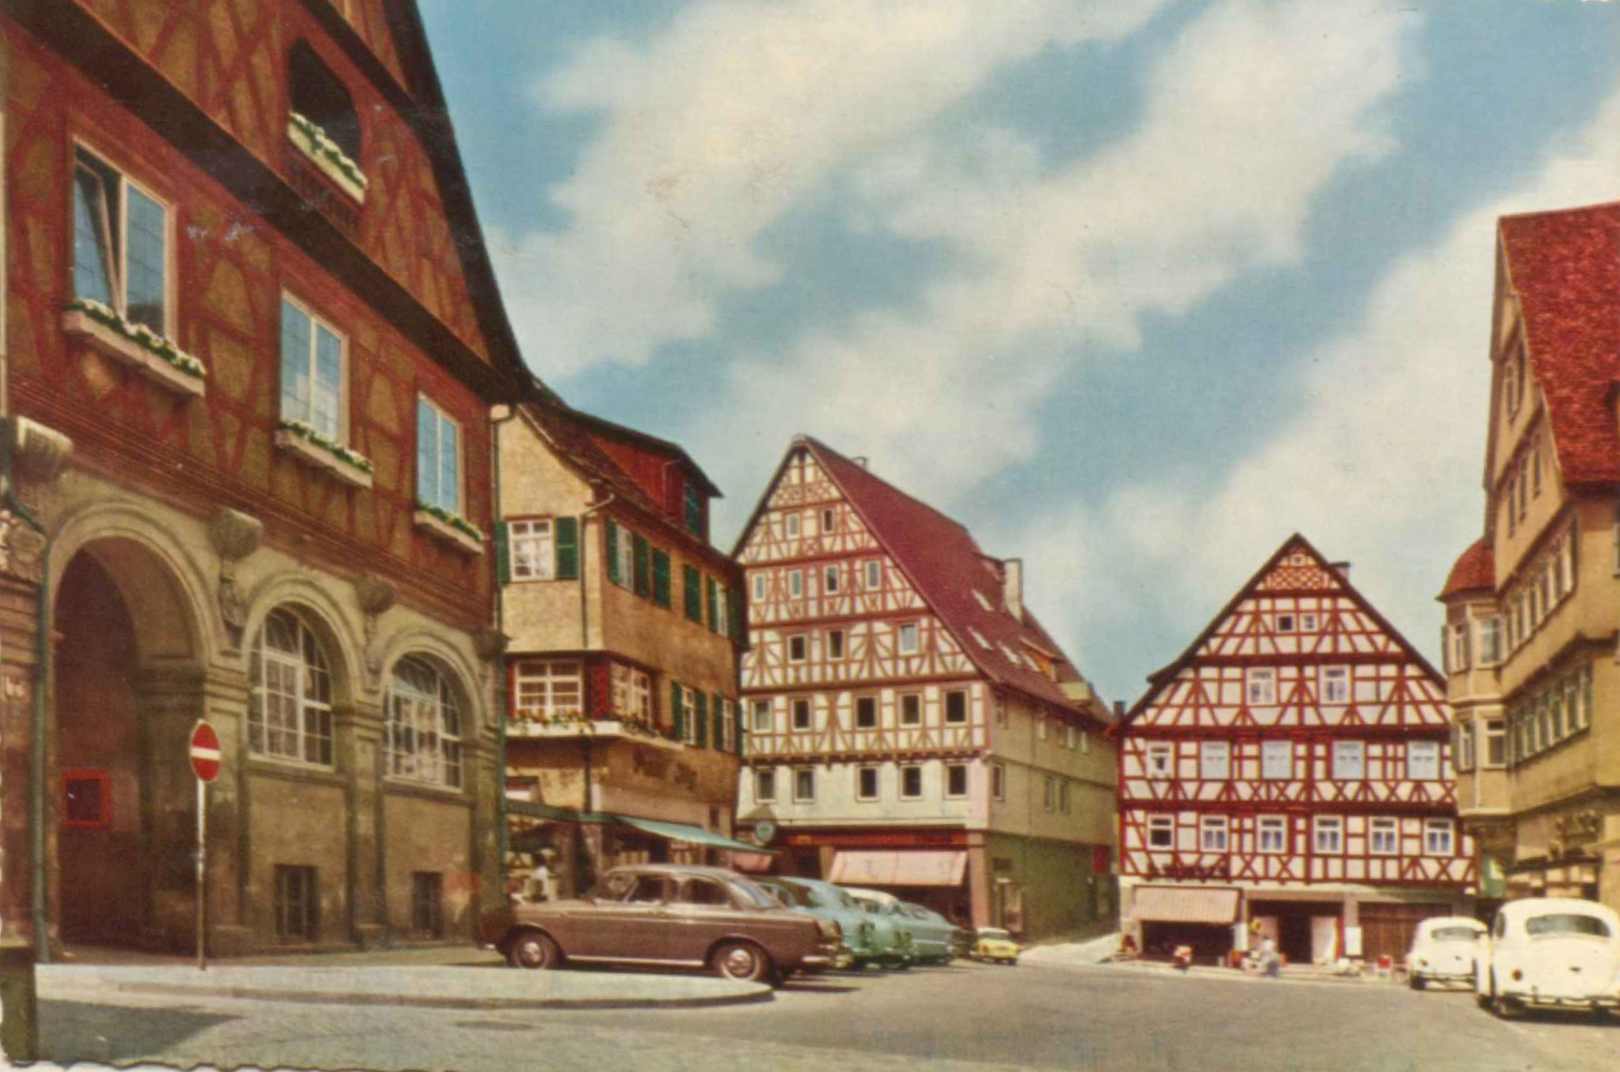
\includegraphics[width=\textwidth, height=\textheight, keepaspectratio]{215-b-waiblingen}
\caption{Rázovité městečko Waiblingen u Stuttgartu. Bydlí zde vnučka Anny Hutterové, rozené Prusíkové z Plas}
\label{fig:215-b-waiblingen}
\end{figure}

% str 187 @ 216 (pokr.)
František Prusík byl až do konce života velmi čilý stařeček. Když jeho třetí manželka v roce 1889 dne 26. ledna v Plasích zemřela, tu zůstal sám, neboť jeho syn Karel byl právě na vandru. Byl by se snad oženil po čtvrté, ale jeho syn se vrátil ze světa, oženil se a dědeček spokojeně dožil uprostřed rodiny svého syna. Zemřel 19. 6. 1902 v Plasích.

Syn Františkův z třetího manželství byl Karel, narozený 22. 10. 1873. Karel Prusík vyučil se košíkářství u Anto­nína Rotta v Plasích. I on se pak jako tovaryš pustil, jako kdysi jeho otec, do světa. Nejdříve pracoval v Děčíně, později přes Plzeň vydal se do Bavor, dostal se až do Solnohradu, kde zase pracoval, pak byl v Innsbrucku, později ve Švýcařich a pak v Mnichově, kde pracoval zas jako košíkář. Odtud musel se vrátil, aby nastoupil dvouletou vojenskou službu a v roce 1896 se opět vrá­til do Mnichova, kde tehdy pracovala jako kuchařka Ludmila Bradáčová, nar. 25. 7. 1872 v Plasích. Ta se pak sta­la jeho ženou. Na naléhání svého otce vrátil se Karel Prusík do Plas a zde založil svou košíkářskou živnost, v níž později tak vynikl. I Karel Prusík psal své pamě­ti jako již jeho otec, které jsou velmi cenným poučením i v dnešní době. Karel Prusík měl pět dětí, čtyři dcery a jednoho syna. Nejstarším dítětem Karla Prusíka a Ludmily roz. Bradáčové, byla dcera Marie. Narodila se 11. 2. 1899 v Plasích a provdala se za dělníka Škodovky Františka Šnábla. Marie Šnáblová žije dnes jako vdova v Plasích č. 33. Měla tři děti. Její syn Jan nar. 10. 1. 1932 zemřel v mladém věku 8. 8. 1948. Dcera Marie nar. 9. 7. 1925 je provdaná Šmídlová. Má dcerku Marii, nar. 14. 3. 1947. Třetím dítětem Marie Šnáblové roz. Prusikové je dcera Ludmila nar. 22. 7. 1937. Je provdaná Třísková a je bezdětná. Žije v Plasích.

Druhou dcerou Karla Prusíka, košíkáře v Plasích je Božena. Narodila se 5. 8. 1900, provdala se za Václava Nového a bydlí v Plasích č. 318. Má dvě děti. Její syn Karel Nový nar. 29. 7. 1926 pracuje v elektrárně a bydlí v Mostě tř. Budovatelů 2365. Má dcerku Hanu nar. 1. 6. 1960. Druhé dítě Boženy Nové roz. Prusíkové je dcera Josefa, narozená 27. 1. 1927. Je provdaná Šandorová a žije v Pla­sích. Její dcera Marie nar. 5. 10. 1946 je nyní provdaná Korbelíková. Má synka Petra nar. 4. 8. 1966. Pavel Šandor je narozen 28. 4. 1949 a bydlí s rodiči v Plasích.

% str 188 @ 217
Jediným synem Karla Prusíka z Plas byl syn Karel. Narodil se 11. 8. 1905. Vyučil se také košíkářskému řemeslu u otce, ale byl také dlouho úředníkem peněžních ústavů, Kampeličky a Spořitelny. Přes třicet let byl náčelníkem Sokola v Plasích, a urči­tou dobu také předsedou Zemské Jednoty košíkářů. Zvláštním jeho koníčkem bylo herectví. V různých rolích vystupoval jako ochotník v obcích rodného kra­je. Nyní žije v Mostě, tř. Budovatelů 2324, kam se uchýlil po roce 1948. Pracoval tam až do důchodu v elektrárně. Za manželku má Anežku Manovou, roz. v Kožlanech 7. 11. 1900. Z tohoto manželství narodily se tři děti. Jeho syn Karel Prusík narodil se 27. 10. 1930 a byl by také převzal živnost košíkářskou, ale vývoj jeho plán zhatil. Nyní pracuje na pile v Plasích, je činným sportovcem a náčelníkem tamního Sokola. Bydlí v Plasích č. 113. Za manželku má Marii Chimincovou nar. 25. 11. 1932 v Záryši na bývalé Podkarpatské Rusi. Mají spolu dvě děti. Dcerka Hana je narozena 6. 4. 1955 a synek Karel 25. 7. 1956. Tento chlapec má jméno Karel již ve čtvrté generaci v rodině a někdy mu proto říkají Karel IV.

Druhým synem Karla Prusíka je Jan. Narodil se 31. 12. 1931. Vystudoval textilní obor v Brně a dnes pracu­je jako textilní mistr v podniku Seba v Dolní Smržovce. Tam bydlí v čísle 1255. Jeho manželkou je rodačka ze Smržovky Marie Endlerová nar. 19. 11 .1940. Jan Pru­sík má dva chlapce. Pavel je narozen 14. 5. 1960 a Jan 2. 7. 1964. Posledním manželským dítětem Karla Prusíka z Plas je dcera Ludmila. Narodila se 17. 6. 1934, vyučila se také v textilním oboru a dělá dnes mistrovou v podniku Benar v Litvínově. Tam bydlí U zámecké zahrady 828.

Karel Prusík má také dvě nemanželské děti. S Věrou Majznerovou z Nové Paky. Je to Milan Majzner nar. 21. 4. 1948 a Věra Majznerová nar. 9. 10. 1951. Tyto děti Karla Prusíka nemají jeho jméno, ale mají krev rodu. Bydlí nyní v Lánech č. 40 u Nové Paky.

Dalším dítětem Karla Prusíka nar. 1873 v Plasích, zakladatele košíkářského podniku, je dcera Ludmila. Narodila se 25. 4. 1907 v Plasích. Měla stejnou lásku k divadlu, jako její bratr Karel a také často hrávala s ochotníky. Vdala se za Františka Čumpelíka do Prahy, ale toto man­želství bylo později rozvedeno. Bydlí v Praze-Nuslích,  U družstva Ideál č. 6. Ludmila Čumpelíková roz. Prusíková měla tři děti. Její dcera Eva nar. 22. 9. 1940 je provdaná Volínová. Bydlí v Praze - Malešicích, Blok 9, č. 362. Má dvě děti. Evu nar. 29. 3. 1960 a Jana nar. 25. 3. 1962. Syn Ludmily Čumpelíkové, Jiří nar. 26. 3. 1944 zdědil asi po matce lásku k umění. Stal se tanečníkem v divadle ABC a také často zajíždí v tomto svém povolání do ciziny. Třetím dítětem Ludmily, roz. Prusíkové je dcerka Jana, nar. 27. 12. 1947. Je bohužel nevyléčitelné nemocná a je v sanatoriu v Černíkovicích u Rychnova nad Kněžnou.

% str 189 @ 218
Posledním dítětem košíkáře Karla Prusíka z Plas byla dcera Helena. Narodila se 29. 1. 1915 a brzy v mládí přišla do Prahy na vychování k Anně provdané Komárkové, jejíž matka byla nevlastní sestrou jejího otce. Helena Prusíková provdala se pak za úředníka Karla Vendra. Bydlí dnes v Praze -Vinohradech,Vinohradská 44. Má dvě děti. Její dcera Věra je úřednicí pražské spořitelny, narodila se 15. 6. 1940 a je provdaná Křenková. Bydlí v Praze l, Klimentská 11. Má dcerku Michaelu nar. 15.  11. 1965, dále Jarmilu nar. 11. 6. 1968. Druhé dítě Heleny Vendrové je syn Karel. Narodil se 19. 1. 1943 a bydlí s rodiči v Praze na Vinohradech. Má synka Romana nar. 2. 10. 1967.

Karel Prusík, zakladatel košíkářské firmy plasské, stal se váženým občanem v Plasích, činovníkem v růz­ných spolcích a svou živnost, v níž velmi vynikl, dovedl daleko. Za druhé světové války zaměstnával 40 lidí a ještě dalších 60 naoko a tím je uchránil od pracovního nasazení do říše. Bohužel po válce do­padl špatně jako všichni živnostníci. Kdyby nebylo jeho dětí, zůstal by býval bez prostředků. Vědomí této závislosti mu ztrpčilo konec jeho života. Umřel v Plasích 8. 12. 1952. Jeho žena, vždy tak pečlivá hos­podyně a matka zemřela brzy za ním dne 5. 5. 1954.

František Prusík, obuvník v Plasích, měl ze svého třetího manželství ještě dceru Josefu. Narodila se 14. 12. 1875. Když jí bylo 19 let seznámila se s Jindřichem Ulvrem, který pracoval jako pekař v Plasích. Provda­la se za něho, když se jí před tím narodil synek Jindřich 28. 11. 1894. Mladí manželé odstěhovali se pak do Dolní Bělé, kde měli pekařství a odtud se zase stěhovali do Kaznějova. Pak se odstěhovala Josefa Prusíková provdaná Ulvrová se svým mužem do Prahy, kde on pracoval jako pekařsky dělník. Po návratu z první svě­tové války najal si Ulvr se svou manželkou zámeckou pekárnu v Praze - Tróji. Bydleli však v Praze 7, v bý­valé Štítného ulici. Až do roku 1949 měla rodina tuto pekárnu. Pak se odstěhovala vdova Josefa Ulvrová roz. Prusíková do Zákup u České Lípy se svou rodinou. Zemřela 5. 2. 1955 a je pochována v Praze-Bohnicích.

Josefa Ulvrová roz.Prusíková měla tři syny a dceru. O jejím prvním synu Jindřichovi jsme se již zmínili. Vyučil se řeznictví a naposled měl svou živnost v Praze-Jinonicích. Byl tam velmi oblíben, což zvláště ukázala veliká účast občanstva na jeho pohřbu. Jindřich Ulvr zemřel 16. 10. 1965.  Měl dva syny. Syn Miroslav nar. 29. 1. 1924 byl také vyučen řezníkem, jako ženatý bydlel ve Stodůlkách u Prahy. Po rozvodu bydlí nyní v Jinonicích. Jeho dvě děti bydlí s matkou ve Stodůlkách. Jsou to dcerka Miroslava nar. 29. 2. 1957 a synek Libor nar. 10. 7. 1959. Druhý syn Jindřicha Ulvra dostal jméno po otci, Jindřich. Narodil se 8. 6. 1932 a je technickým úředníkem. Bydlí v Praze Jinonicích, Karlštejnská 28, kde míval jeho otec živnost. Má dvě děti. Syna Michala, nar. 16. 10. 1957 a dcerku Zuzanu nar. 1. 9. 1961. Miroslav Ulvr zemřel 2. 2. 1969.

% str 190 @ 219
Druhým dítětem Josefy Ulvrové, roz. Prusíkové je Václav. Narodil se 17. 8. 1898 v Dolní Bělé u Plas. Dnes žije v Zákupech, Kamenická 76. Měl nemanželského syna Břetislava, který má jméno po matce, Košťál. Je narozen 15. 9. 1929 a bydlí v Praze 7,  Poupětova, 11. Je v podniku Vihorlat a nadšeným zpěvákem. Ze svého manželství má Václav Ulvr ještě syna Jindřicha, který se narodil 21. 11. 1941. Pracuje ve staveb­nictví a bydlí v Praze 4-Bráníku, Novodvorské sídliště č. 1165. Má dcerku Janu Ulvrovou nar. 16. 6. 1963. Třetím synem Josefy Ulvrové byl Vilém. Narodil se 26. 1. 1900 a byl pekařem a tuto svou živnost provozoval až do roku 1949, kdy se odstěhoval do Zákup. Byl bezdět­ný a zemřel 27. 10. 1939.

Josefa Ulvrová roz. Prusíková měla dceru Marii. Narodila se 3. 7. 1902 v Dolní Bělé. Pak se stěhovala s rodiči do Kaznějova a do Prahy a vdala se za Josefa Syrovátku. Ten měl první výrobu dětských kočárků v Praze-Hole­šovicích. V důsledku hospodářské krise byl nucen pod­nik uzavřít a pracoval pak jako dělník. Marie Syrovátková měla dva syny, kteří dospěli. Syn Alois narodil se 21. 7. 1921 a vyučil se řeznictví. Jeho zálibou byl řecko-římský zápas, ve kterém vynikl. Alois Syrovátka a pak i jeho bratr Jindřich zápasili v košířském klubu A. K. Hellas. V roce 1946 stal se profesionálem a do­byl titulu mistra ČSR a Prahy. Předtím, jako amatér byl mistrem Čech a Moravy. Alois Syrovátka bydlí ve Velenicích u Zákup č. 80. Má dvě děti. Olgu nar. 8. 9. 1943, která je provdaná Součková. Je vyučenou tkadlenou. Má synka Miroslava nar. 25. 11. 1963. Druhou dcerou Aloise Syrovátky je Miroslava, nar. 7. 8. 1946. Druhý syn Marie Syrovátkové je Jindřich. Narodi1 se 2. 6. 1923 v Praze. Byl vyučen pekařem, ale nyní jako jeho bratr Alois je řidičem v mlékárně v Zákupech. Jindřich je ženatý, ale nemá vlastní děti. Bydlí v Zákupech, Kamenická 88. Matka jejich Marie Syrovátková roz. Ulvrová bydlí ve Velenicích č. 56 u Zákup.

To byl tedy popis života všech potomků Františka Prusika, obuvníka z Plas, který se narodil 1823 v Nebřežinech. Přesto, že byl prostým obuvníkem, byl velmi inteligentním člověkem a pamětníkem mnoha pohnutých událostí ve svém rodišti v Nebřežinech a v Plasích, kde zemřel.

Druhým synem Josefa Prusíka, obuvníka v Nebřežinech byl Josef. Narodil se 8. 10. 1826 a brzy odešel do Prahy. Velkou pílí domohl se zde pěkného postavení. By1 nejdříve menším úředníkem, ale pro svou snahu a znalosti rychle postupoval. Po večerech se kromě tehdy běžné němčiny naučil i francouzštině a italštině a stal se brzy účetním a později prokuristou u tehdy velmi známé firmy Wimmer. Rodina tato patřila mezi přední patricijské rody v Praze. Jejich předek zbohatl na státních vojenských dodávkách, postavil pěkné domy a rodina Wimmerů budovala i parky, kašny a ve svých salonech na tehdejší Ferdinandově třídě (Národní) hostila ruského generála Suvorova.

% str 191 @ 220
Když přisel Josef Prusík z Nebřežin do Prahy, byla již národně probuzená. Tvořily se spolky s národním zaměřením, zakládaly se nové živnosti, manufaktury, které začaly dobře prosperovat a vůbec celý národní a hos­podářský život v Praze dostal prudký spád. Nebylo daleko před revolučním rokem 1848. Přestože Josef Prusík pracoval u firmy, která byla německého zaměření, zůstal on věrným Čechem, poznal se s mnoha vynikajícími lidmi, zvláště s herci a hudebníky z Prozatímního divadla. Z Prusíků v té době byl Josef Prusík vedle kněze Blažeje Prusíka jediný, kdo žil tehdy v tomto národně kvasícím městě. Prokurista Josef Prusík znal se s Bedřichem Smetanou, kapelníkem Čechem z Národního divadla a s mnohými herci, patřícími k tak zvané staré gardě Národního divadla. Účastnil se i bouří svatodušních v roce 1848 a za dvacet let později zase slavného položení základ­ního kamene k Národnímu divadlu.

Josef Prusík oženil se s měšťanskou dcerou Františkou Šulákovou nar. v Praze 9. 4. 1832. Bydlili v Praze 1, Rytířská ul. 402. Svatbu měli v roce 1851. V tomto manžel­ství narodily se jim tři děti. První byla dcera Marie, nar. roku 1852, která se pak provdala za inženýra Hrnčí­ře. Měli jednoho chlapce Zdeňka nar. 1876, který však již ve dvanácti letech zemřel a to 17. 2. 1888. Tuto ztrátu Marie Hrnčířová velmi těžce nesla, dětí pak již nemě­la a zemřela 1. 2. 1900 v Praze.

Josef Prusík zemřel 31. 8. 1895 a jeho manželka ho přeži­la o dvacet let, zemřela 7. 7. 1915. Jsou pochováni na Olšanech, blíže hrobu malíře Čermáka.

Druhým dítětem byl syn Josef. Narodil se 21. 4. 1855 a stal se úředníkem. Působil u různých firem jako účetní a pak dlouhou dobu v podniku, kde již byl jeho otec, u firmy Wimmer. Bydlel v témže bytě v Rytířské ulici jako již jeho otec a je zajímavé, že ještě v jarních měsících roku l968 bydlí tam jeho vdova. Je jistě málo ta­kových případů v Praze, aby v témže bytě a domě bydlel nájemník a jeho potomci nepřetržitě 120 let. Josef Prusík byl dvakrát ženat. První jeho manželkou byla Barbora Svobodová, nar. 31. 1. 1857 v Praze. Zemřela 11. 8. 1919. S druhou manželkou Annou roz. Hemalovou z Brna, kde se narodila 10. 6. 1892, nežil však dlouho.

Josef Prusík měl vedle svého zaměstnání mnoho různých zálib. Výborně maloval, dovedl si ušíti boty a zhotovil si i gramofon. Elektřina byla zvláštní jeho zálibou, ale rádia se vlastně nedočkal. Zemřel náhle 18. 6. 1924 v Praze a byl pochován na Olšanech. Josef Prusík měl z prvního manželství pouze dvě dcery, z druhého manželství děti neměl.
První dcera Josefa Prusíka, Františka narodila se v Úvalech, kde její rodiče jeden čas bydleli, 24. 1.  1880.
% str 192 @ 221
Zemřela po zápalu plic, svobodná ve svých 22 letech 9. 11. 1902 v Praze.

Druhou dcerou byla Adéla. Narodila se 9. 10. 1884 provdala se za nájemce statku v Hrdlořezech, Josefa Zunu. Později její manžel působil na pražských jatkách jako komisionář. Adéla Zunová, roz. Prusíková měla syna a dceru. Zemřela v Praze 5. 12. 1952. Je pohřbena v hrobce svých rodičů, na Olšanech.

Syn Adély Prusíkové, provdané Zunové je Vilém. Narodil se 11. 4. 1910, byl také dlouho komisionářem na pražských jatkách, ale od roku 1945 pracuje v obchodě. Bydli v Praze - Podolí, Na dolinách 7. Má dceru Moniku nar. 22. 10. 1946.

Druhým dítětem Adély Zunové roz. Prusíkové byla dcera Valerie. Narodila se 28. 8. 1912 v Praze a je provdaná Borůvková, bydlí v Praze - Podolí, Na dolinách 23. Je bezdětná. Pracuje jako úřednice v ROH, odbor bezpečnosti práce. Jak Vilém, tak i Valerie nezapomínají nikdy, že patří po matce k rodu Prusíků a k němu se také vždy hlásí.

Třetím dítětem Josefa Prusíka, který přišel z Nebřežin do Prahy v první polovině XIX. století, byla dcera Františka. Narodila se 17. 8. 1860 a poprvé provdala se za velkoobchodníka Josefa Kováře. Manželství trvalo 17 let. Z tohoto manželství narodila se dcera Františka 6. 5. 1880. Provdala se za úředníka Bozděcha, který byl později mi­nisterským radou ve Vídni a po převratu 1918 na ministerstvu veřejných prací v Praze. Františka Bozděchová bydlí dnes v Praze Košířích, Plzeňská 47. Její velkou zálibou býval zpěv, měla i nabídky divadel ještě když žila ve Vídni. Tam zpívala na kůru ve svatoštěpánské katedrále. Uchovává pietně památky na svou matku i děda, Josefa Prusíka, jehož malovaný portrét visí v jejím bytě. Má jediného syna Alexandra Bozděcha. Narodil se 5. 4. 1902 ve Vídni, vystudoval práva, měl svou vyhlášenou advokátní kancelář v Praze a nyní pracuje ještě v advo­kátní poradně. Dr. Alexandr Bozděch je svobodný.Ve své funkci s výbornou znalostí cizích jazyků často zajížděl do ciziny. Bydlí s matkou v Praze - Košířích.

Františka Kovářová, roz. Prusíková se brzy po ovdovění provdala za lékárníka Lamače. S ním měla jediného syna Karla, který se narodil 28. 1. 1897 v Praze-Košířích. Zemřel 2. 8. 1922 v Hamburku, kde je pochován. Jeho maminka, Františka Lamačova roz. Prusíková zemřela ve vysokém věku 89 let dne 3. 9. 1949 a je pochována na hřbitůvku v Košířích (Kotlářka). Nyní si něco povíme o Karlu Lamačovi, který po matce patří zjevně k našemu rodu Prusíků.

% str 192+1 @ 222
\begin{figure}
\centering
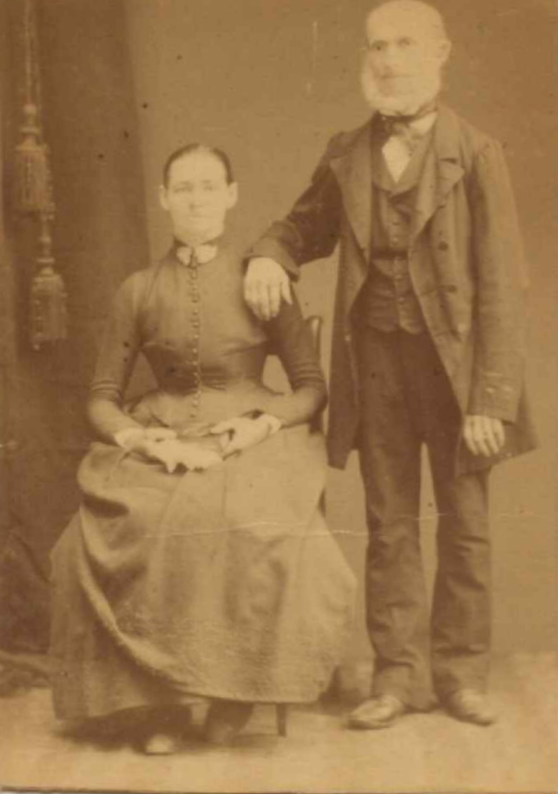
\includegraphics[width=\textwidth, height=\textheight, keepaspectratio]{222-a-frantisek_prusik-1823}
\caption{František Prusík, narozený 1823 v Nebřezinech, usazený v Plasích (1823 – 1902)}
\label{fig:222-a-frantisek_prusik-1823}
\end{figure}

             \begin{figure}
\centering
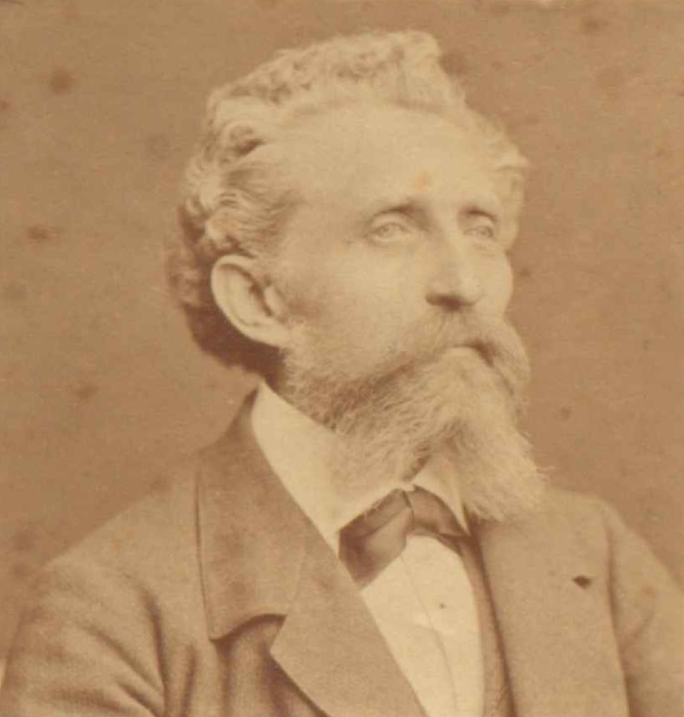
\includegraphics[width=\textwidth, height=\textheight, keepaspectratio]{222-b-josef_prusik_1826}
\caption{Josef Prusík, bratr Františkův, nar. 1826 v Nebřezinech a usazený v Praze (1826 – 1895)}
\label{fig:222-b-josef_prusik_1826}
\end{figure}

\begin{figure}
\centering
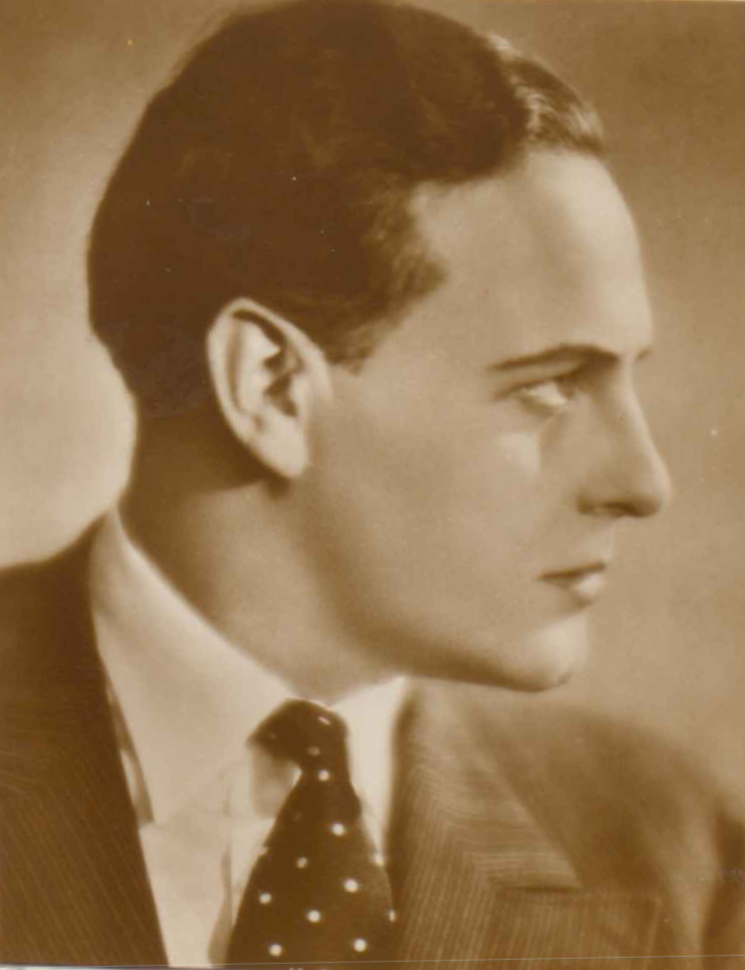
\includegraphics[width=\textwidth, height=\textheight, keepaspectratio]{222-c-karel_lamac}
\caption{Vnuk Josefa Prusíka Karel Lamač, průkopník českého filmu (1897 – 1952)}
\label{fig:222-c-karel_lamac}
\end{figure}


% str 192+2 @ 223
\begin{figure}
\centering
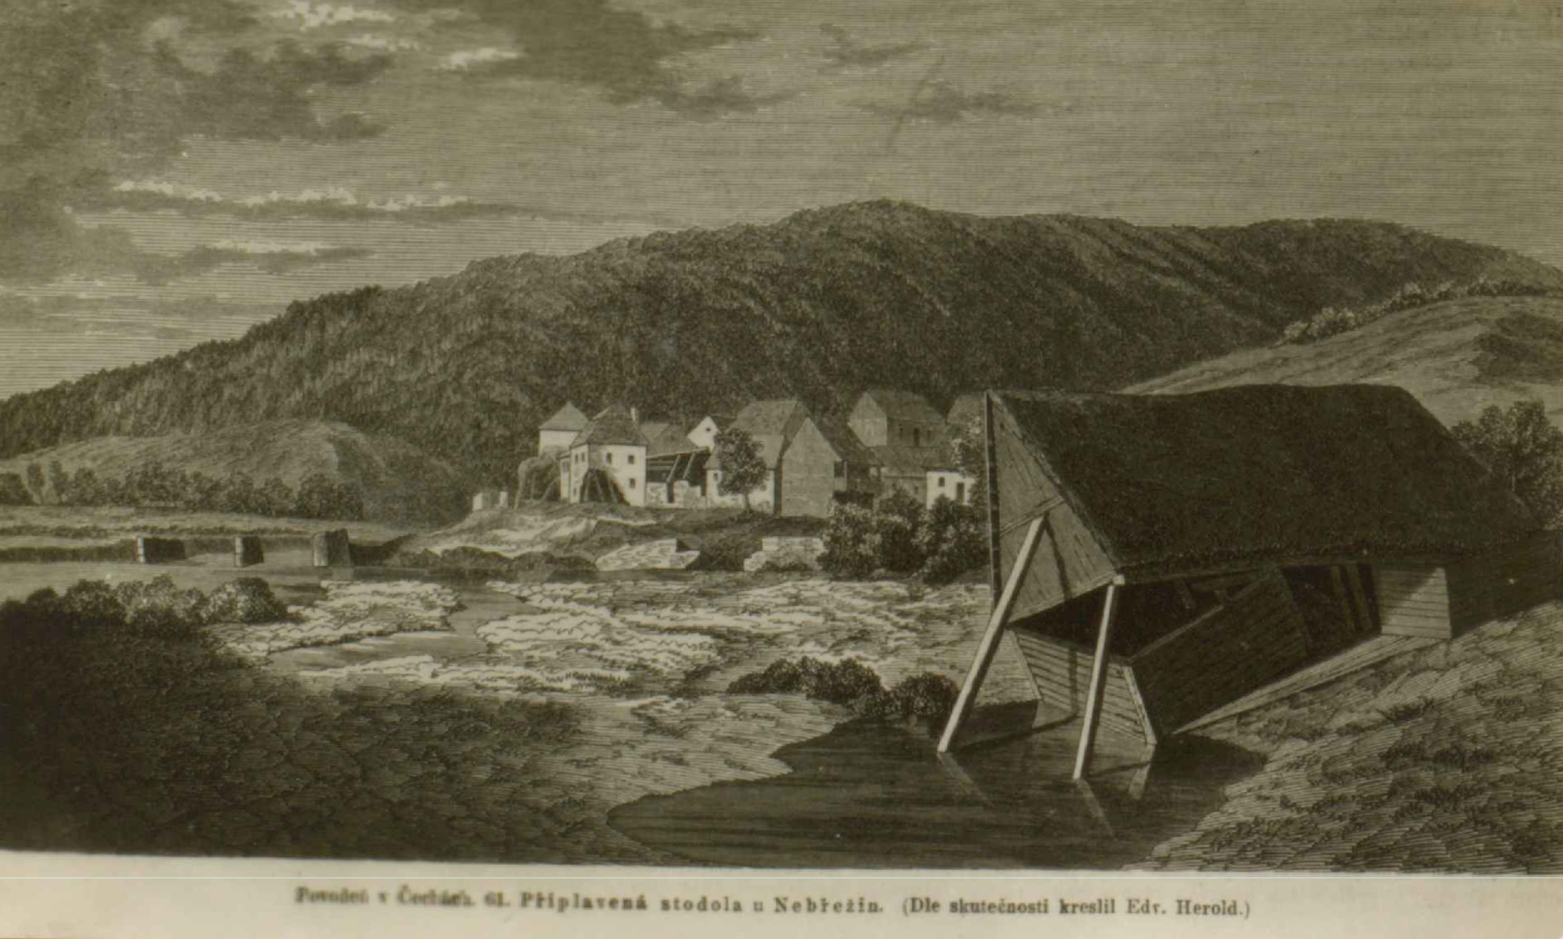
\includegraphics[width=\textwidth, height=\textheight, keepaspectratio]{223-povoden_v_nebrezinech}
\caption{Při povodni 25. května 1872 zahynuli mezi 62 lidmi v Nebřezinech u Plas i četní členové rodu Prusíků a také zázračně zachránila se jako plovoucí v kolébce na řece Marie Prusíková, narozená 1870, později provdaná Paclová v Plzni, kde zemřela ve věku 80 let v roce 1950}
\label{fig:223-povoden_v_nebrezinech}
\end{figure}


% str 193 @ 224
\section{Karel Lamač, průkopník českého filmu}

Když se 28. ledna 1897 narodil Karel Lamač, zapisoval ho v košířském kostele při křtu do matriky pan farář, a tu jeho otec lékárník Lamač uzřel, že nad konečným písmenem c není háček. Zaprotestoval nesmělým hlasem: "Nezlobte se, důstojný pane! Chyba! Prosím, tam na konci toho jména musí být háček Lamač, ne Lamac!" Jakmile se novorozeně postavilo na vlastní nohy, což bylo ve věku asi 25 let, stalo se filmovým hercem a pak postupem doby známým českým a později i meziná­rodním filmovým režisérem: Musel v tom být vždycky há­ček! A to nejen doma, ale i v cizině. V cizině v tom ovšem byl háček, když v tom měl být háček, neboť v ci­zině si na háčky moc nepotrpěli. Avšak Karel Lamač byl důsledný a kolují celé zvěsti o tom, jak všude v Německu, Rakousku, Anglii, Holandsku, Francii, Americe, všude tam, kde režisér Karel Lamač působil, s houževnatostí a tvrdostí pro cizince nepochopitelnou, trval na háčku na c. Často Lamač vyhrožoval zákazem předvá­dění, nebude-li titulek správně předělán. Poprvé to by­lo v Berlíně před předváděním veselohry Polní maršálek v kině Atrium. Lamač nepovolil a háček na konci jména musel být. Hrstka Čechů, která přijela na předvádění z Prahy, měla z toho radost a uspokojení. Něco podobné­ho dálo se pak s jeho jménem v Mexiku, Paříži a jinde. Vždy se však jméno Karel Lamač skvělo na bílém plátně správné a v plné slávě.

Za svůj poměrné krátký život natočil Karel Lamač jako režisér přes 200 filmů. Pamatují se ještě dobře jeho filmy Kantor Ideál, Polní maršálek, Bílý ráj, Chyťte ho! Osudy dobrého vojáka Švejka a jiné.

Karel Lamač studoval původně farmacii a chemii, ale film ho pak odtáhl od studií a proslavil. Jako technik, chemik, optik, badatel v oboru filmu, učinil řadu objevů, které pomáhaly vývoji světové kinematografie. Jako vynálezce se bude jednou připomínat v oboru fotografie, gramofonu a zvukové techniky, jako konstruktér v oboru kamery, telefonu a osvětlovací techniky. O Karlu Lamačovi říkají přátelé, že to byl člověk, který nikdy nikoho nezarmoutil. V hlavních městech Evropy byl znám v ateliérech a kavárnách umělců, i v kancelářích patentních a právních znalců. U berlínského krejčího si objednával oblek, v Praze platí dluh jinému, ve Vídni dostává oblek do hotelu ušitý, který si loni objednal a zapomněl odebrat a nyní je mu malý. Všude má přátele a všude věři­tele. Nikde nemá klid. Neví co je to soustředění. Dokončí jeden film a usíná ve spacím voze nad libretem, které má začít filmovat podle smlouvy na konečná stanici a dosud neměl čas ani si přečíst název.

Martin Frič vzpomíná na Karla Lamače takto: "Pro mne Červená sedma a Eduard Bass to byli bohové. Chodil jsem tam a dokonce jsem se stal členem kabaretu. Tehdy byl
% str 194 @ 225
kabaret něčím novým, byl to zlom ze šantánu, nový vítr asi jako dnes avantgardní divadla. Za dva roky na to nastoupil film, to byly tenkrát dvě novinky. K filmu se vždycky ze začátku stahovali podvodníci, takoví, co slibovali hokynáři, že dceruška bude ve filmu, když jim půjčí. Díky jim, měl film strašnou pověst. Já měl štěstí, že jsem se od počátku spojil s Karlem Lamačem, prvním z poctivých filmařů. Že jsem k němu měl oprav­dový vztah, to snad dokládá ten fakt: Když přišel zvuk, nechal jsem natáčení, rok jsem se učil u Lamače v Pa­říži stříhat zvukový film, pracovat se zvukovou apara­turou a teprve pak jsem se vrátil za kameru a začal natáčet Švejka."

Karel Lamač tedy je u nás první, kdo zavedl zvukový film a technice s ním rozuměl. V rohovém pokoji ve svém košířském bytě s výhledem na hřbitov měl Karel Lamač postel. Na ní bylo plno knih, tlustých slovníků, drátů, rámečků, obrázků, rozvinutých filmů, nákresů a žárovek a ovšem pak bylo málo místa na loži pro ramenatého muže s antickým profilem. V poloze ležmo Karel Lamač odpočíval jako staří Římané, přemýšlel, psal, telefo­novat po celé Evropě, v leže řešil složité finance, jedl, spal a vždy říkal, že jen v leže může filmař klidné snášet příkoří producentů, podnikatelů a jiných darebů s penězi a bez peněz.

Karel Lamač, který ze studia farmacie a chemie přesedlal na optiku a slaboproudou elektřinu, byl pak spisovatelem, hercem, badatelem, režisérem, vynálezcem, manipulátorem a kouzelníkem, pianistou, ale především filmařem. Na to, aby se oženil neměl nikdy čas. Karlíček, jak mu jeho druhové říkali, stále něco vynalézal, ale proti Zubaté nevymyslel nic. Šťasten býval u své maminky, která patřila do rodu Prusíků. V pokoji nad starou lékárnou hledíval oknem do rozkvetlé a zpěvem ptactva naplněné „zahrady zelené" zeleně stromů starého košířského hřbitova. A dole v lékárně jeho otec, kdysi znamenitý zpěvák a bývalý první tenor Národního divadla, jeden z prvních Jeníků v Prodané nevěstě, mísil lektvary, prášky, odpočítával kapky a odvažoval dávky.

Karel Lamač vracel se z Ameriky do vlasti a tu ho volala jeho věrná spolupracovnice z mládí Anna Ondráková, že podniká film a chce mu svěřit vedení. Seděl nad psacím strojem a rozepsanou filmovou komedií z pařížských musichallů a tu ho překvapila smrt. Bylo to 2. srpna 1952 v Hamburku a tam byl pochován.

Jeho české jméno na náhrobním kameni s háčkem na posled­ním písmeně hlásá, že pro každého na tomto světě platí věčně slova: "Rozkazem obracíš člověka v prach a říkáš: Vraťte se, lidské děti!"

% str 195 @ 226
Z dětí Josefa Prusíka, obuvníka v Nebřežinech jediným "pánem" stal se tedy Josef Prusík, který žil v Praze. Jeho dcera Josefa měla dělníka, Marie rovněž, Alžběta zůstala svobodná a nežila doma v žádném nadbytku a František byl ševcem. A poslední syn Emanuel stal se slevačem.

% ________
Emanuel Prusík, poslední dítě Josefa Prusíka v Nebřežinech, který tam přišel v roce 1816 z Plas, narodil se 5. 1. 1832. Kníže Metternich zřídil při svém panství v Plasích železářskou huť a tam, kde stála, říká se ještě dnes na verku. Huť zaměstnávala dosti značný počet lidí a Emanuel Prusík stal se tam také dělníkem. Výrobky této slévárny je možno vidět ještě dnes v kraji zvláště na hřbitovech. Emanuel Prusík oženil se s Barborou Šrédlovou, která pocházela z Obory u Liblína a narodi­la se tam v roce 1825. Byla tedy starší o sedm let než její muž. Emanuel s Barborou měli několik dětí, ale hodně jich umřelo v dětství. Dospěl jen syn František a dcera Josefa. Emanuel Prusík neměl lehký život, zemře 28. 3. 1894 v Plasích. Ačkoliv byl nejmladší z bratrů, zemřel první. Bydlel celý život v Nebřežinech a zažil tam zhoubnou povodeň, před níž se však zachránil. Jeho žena zemřela 8. 12. 1907 v Nebřežinech.

Syn Emanuela Prusíka byl František. Narodil se 22. 12. 1852 v Nebřežinech a byl tak zvaným mlynářským v chemické továrně J. D. Starcka v Kaznějově. Manželkou jeho byla Viktorie Šístková nar. v roce 1860 v Nebřežinech, kde zemřela 11. 11. 1932. František Prusík postavil si v Nebřežinech domek a továrník Starck, když došlo jednou ke stávce jeho dělnictva, poukazoval na to, jak se jeho zaměstnancům dobře daří, že si i při velkém počtu dětí mohou postavit pěkný domek. František Prusík říkal kaž­dému vše otevřeně do očí, ale při tom byl v okolí velmi oblíben pro svou poctivost. Zemřel v Nebřežinech 24. 2. 1923. Svatbu měl v roce 1897 než se mu narodilo poslední dítě. Do té doby žil se svou ženou neoddán, ale velmi šťastně.

Prvním synem Františka Prusíka byl Jan. Narodil se 26. 2. 1878 v Nebřežinech, č. 35. Byl kovářem, jeden čas v Kaznějově a pak v Dnešicích u Přeštic. Za manželku měl Marii Mertlovou nar. 3. 5. 1880 v Korytech u Plas. Kovář Jan Prusík zemřel v Dnešicích 8. 8. 1958 a jeho žena ho následovala do hrobu za necelý rok 8. 7. 1959. Měli spo­lu tři děti, dva syny a dceru.

Nejstarší byl Jaroslav nar. 14. 11. 1907 v Kaznějově. Byl technickým úředníkem naposled v Chlumčanech u Dobřan v Kaolinových závodech. Pro své schopnosti dostal tovární titul inženýr. Zvláštní jeho zálibou byla hudba. Byl kapelníkem souboru a také rád sledoval historické a archeologické památky. Byl také dobrým znalcem života všech potomků pradědečka Emanuela Prusíka. Zemřel bohu­žel mlád v 52 letech dne 10. 7. 1959 v nemocnici v Klatovech. Příčinou byla rakovina plic a jiné neduhy, zvláště slabé srdce. Za manželku měl inž. Jaroslav Prusík Marii
% str 196 @ 227
Červenkovou, nar. 10. 8. 1912 v Dolní Lukavici. Ta bydlí v Chlumčanech u Dobřan č. 320. Jaroslav Prusík se svou chotí Marií měli tři dcery a syna. Nejstarší je Jaroslava nar. 18. 4. 1932, je provdaná Veinfurtová a bydlí v Chlumčanech č. 218. Je úřednicí. Za manžela má technického úředníka Veinfurta ve Škodovce. Mají synka Jaroslava nar. 29. 1. 1958. Druhá je Libuše, nar. 1. 7. 1937. Pracuje jako úřednice v podniku Restaurace a jídelny. Jejím manželem je úředník Ladislav Kumpa. Bydlí ve Staňkově, Nádražní 90. Mají dcerku Libuši nar. 27. 2. 1954. Třetí dcerou je Miloslava nar. 2. 6. 1940. Provdala se za kuchaře Eduarda Hebedu. Sama je úředni­cí. Bydlí v Plzni Sladkovského 67.  Mají dvě děti. Synka Eduarda nar. 9. 6. 1961 a dcerku Martinu, nar. 19. 5. 1966. Posledním dítětem inž. Jaroslava Prusíka z Chlumčan je syn Jaroslav nar. 6. 4. 1951. Bydlí s matkou v Chlumčanech.

Druhým dítětem Jana Prusíka byla dcera Amalie. Narodila se v Dnešicích 18. 6. 1910 a provdala se do Chlumčan za Antonína Žemličku, měla dvě děti. Její syn Miroslav Žemlička je drogistou a žije v Chotěšově č. 475. Narodil se 1. 6. 1931. Má dceru Věru nar. 24. 2. 1959 a Mirosla­vu nar. 23. 5. 1964. Pak měla Amalie ještě dceru Ivu Žemličkovou, nar. 18. 4. 1948. Bydlí v Chlumčanech č. 147. Bohužel po tomto dítěti začalo se Amalii zatemňovati vědomí a od roku 1950 je v ošetřování psychiatrické léčeb­ny v Dobřanech.

Posledním dítětem Jana Prusíka je syn František, Vladislav Prusík. Narodil se 31. ledna 1914 a bydlí v Dnešicích čp. 145. Je soustružníkem. Jeho manželka Marie je rozená Kadlecová z Dnešic, 17. 1. 1919. Mají dva syny. Vladimír Prusík je narozen 30. 12. 1946, je dělníkem a jako ženatý žije v Černotíně u Dnešic č. 36. Manželkou jeho je Jindřiška Kůsová nar. 8. 1. 1951. V době, kdy sestavujeme tyto dějiny rodu je nejmladší manželkou Pru­síka na světě. Druhý syn Františka je Vladislav. Narodil se 17. 3. 1953 a bydlí v Dnešicích s rodiči. Vladimír Prusík má synka Vladimíra nar. 29. 5. 1968. Je to nejmladší Prusík. Druhým dítětem Františka Prusíka z Nebřežin byla dcera Magdalena. Narodila se 27. 4. 1880. Byla švadlenou a zemře­la svobodná 12. 11. 1917 v Nebřežinech.

Dalším dítětem Františka byla Marie. Narodila se 13. 4. 1883 a jejím manželem byl dělník Josef Skočil z Plas. Také ona měla krátký život. Zemřela 14. 2. 1921. Zachoval se po ní syn Josef a i jeho osud byl špatný. Ostatní dě­ti Marie Skočilové zemřely v dětství. Josef Skočil na­rodil se 16. 2. 1906 v Plasích. Za druhé světové války musel odejít do říše a tam zemřel v Řezně 24. 4. 1943. Zanechal dcerku Květu nar. 7. 3. 1931. Ta je dnes provdaná Soukupová a žije v Mladoticích č. 103. Má dvě děti. Vladimíra Soukupa nar. 21. 12. 1954 a dcerku Hanu nar. 18. 8. 1959.

Druhým synem Františka Prusíka byl František. Narodil se 20. 12. 1885 a byl zedníkem. Z první světové války vrátil se jako ruský legionář. Žil v Dnešicích u Přeštic.

% str 197 @ 228
František Prusík byl dvakrát ženat. První jeho ženou byla Barbora Urbánková nar. 24. 5. 1889 v Nebřežinech. S ní měl František dcerku Marii nar. 7. 9. 1913. Její matka zemřela již týden po porodu 14. 9. 1913. Otec odešel do války a tak se jí ujali dědeček a babička se strany otcovy. Svého tatínka poznala až po válce. Marie se provdala za Josefa Kotta do Horní Lukavice čp. 90. Mají dcerku Evu nar. 4. 12. 1946. Než odjel do války oženil se František Prusík po druhé. Jeho manželkou byla Antonie Bendová nar. 10. 5. 1884, v Dnešicích. Z tohoto manželství narodil se syn František 2. 10. 1914. Je instalatérem a bydlí v Dnešicích čp. 54. Za manželku má Anežku Kulišánovou nar. 28. 9. 1915 ve Lhovicích u Švihova. Mají spolu tři děti. Syn Fran­tišek je narozen 31. 1. 1946, dcera Marie 30. 9. 1950 a Anna 4. 7. 1952.

Zedník František Prusík byl v Dnešicích velice oblíben a byl to opravdu řádný muž. Zemřel 24. 7. 1959 a jeho manželka tentýž den. Svou životní pouť ukončili u dcery v Horní Lukavici.

Dalším dítětem Františka Prusíka, narozeného v roce 1852 v Nebřežinech, byla dcera Anna. Narodila se 12. 7. 1888 a provdala se za dělníka, vdovce Václava Janouškovce v Litém u Dolní Bělé. Manželství její bylo bezdětné. Zemřela 28. 7. 1934.

Syn Františkův, Jaroslav Prusík, narodil, se v Nebřežinech 30. 4. 1893. Byl vyučen kovářem. Přiženil se do Babiné u Plas. Jeho manželkou byla Anežka Smetáková, narozená tam 24. 1. 1895. Z manželství se narodily dvě děti, syn a dcera. Toto manželství se pak později nevydařilo z různých důvodů. Jaroslav Prusík se nakonec odstěhoval a o děti se již nestaral. Také alkohol byl jeho zlým druhem. Oženil se po druhé a usadil v Kynšperku nad Ohří. Odtud se odstěhoval, když prodal svůj domek, do Pňovan u Plzně. Zemřel 4. 8. 1966. Jeho druhou manželkou, s níž však již neměl děti, byla Antonie Hejná, narozená 27. 8. 1894 v Dobevi u Písku. Žije v Pňovanech č. 3. u Plzně. Ze svého prvního manželství má dceru. Jaroslav Prusík měl ve svém prvním, nepodařeném manželství syna Ladislava. Narodil se 10. 2. 1920. Byl kovodělníkem a pracoval nejdříve ve Škodovce v Plzni. Později se přiženil do Výrova-Hadačky, kde si vzal tamní rodačku Boženu Opatovou, která se narodila 13. 7. 1922.  Ladislav Prusík se stal členem JZD ve Výrově a pěkně si zvelebil svůj domek. Nyní pracuje v Kaznějově. Má 4 děti. Bydlí v Hadačce č. 38. Nejstarší je dcera Jana. Narodila se 16. 8. 1943 a je dnes provdaná Svobodová v Horní Bříze č. 117. Má dvě děti: synka Jaromíra nar. 15. 5. 1961 a dceru Janu nar. 11. 6. 1962. Druhá dcera Ladislava Prusíka z Výrova, rodáka z Babiné, je Jaroslava. Má za manžela Oldřicha Klinkovského, technika Spojů. Mají dcerku Ivettu. Jaroslava Prusíková, provdaná Klinkovská na­rodila se 14. 11. 1945 a její dcera 25. 12. 1964. Bydlí v Praze 10 Na Hroudě, 2121. Starší syn Ladislava je po otci Ladislav. Narodil se 28. 5. 1948 a je dělníkem. Druhý Josef Prusík nar. 8. 1. 1953 bydlí ve Výrově s rodiči. Oba jsou zpěváci a  účinkovali často v různých souborech.

% str 198 @ 229
Druhým děckem Jaroslava Prusíka z Babiné u Plas byla dcera Blažena. Narodila se 7. 3. 1922. Manželem jejím stal se dělník Škodovky Jaroslav Beneš. Bydli v Babiné č. 34. Blažena Prusíková provdaná Benešová, má dceru Hanu narozenou 19. 8. 1946. Ta je nyní provda­ná Spěváková a má synka Pavla nar. 6. 8. 1967.

Poslední dcerou Františka Prusíka z Nebřežin byla Josefa. Narodila se 19. 9. 1895 a zůstala v domku, který její otec postavil v Nebřežinech. Provdala se za bystrého a hodného člověka horníka Emanuela Bendu. Měli spolu několik dětí, z nichž tři dospěly. Josefa Bendová, rozená Prusíková žila po smrti svého manžela u své dcery v Bochově. Byla to veselá a velmi pracovitá žena. Zemřela 21. 2. 1968.

Její nejstarší dítě je dcera Emilie. Narodila se 22.  2. 1920 a vzala si dělníka Václava Rambouska. Toto manžel­ství mělo někdy své disharmonie, bylo rozvedeno a za­se k vůli dětem se rozvedení manželé znovu vzali. Jejich syn Václav, narozený 25. 3. 1940 pracuje v důlním průmyslu a bydlí v Nýřanech u Plzně, Nové sídliště č. 392. Má dva synky, Milana nar. 22. 6. 1959 a Ivo Rambouska nar. 9. 6. 1962. Druhý syn Emilie Rambouskové je Miloslav. Narodil se 19. 8. 1943. Žije s matkou v Bochově č. 181. Emilie Rambousková vyrostla z chudých poměrů, ale má značnou inteligenci. Ráda píše zdařilé básně.

Druhou dcerou Josefy Bendové, roz. Prusíkové byla dcera Viktorie. Narodila se 31. 12. 1921 a provdala se za dělníka Antonína Krista z Kaznějova. Bydlí tam v čísle 221. Její muž pracuje v tamním průmyslu a je velmi činným odborovým pracovníkem. Mají dvě děti. Jiří se narodil 2. 10. 1945 a Naděžda 12. 8. 1947. Jiří pracuje a bydlí v Mladé Boleslavi. Třetím dítětem je Josef Benda. Narodil se 16. 3. 1925. Pracuje a bydlí v Chebu, Palackého 19. Má dvě děti. Syna Milana nar. 25. 1. 1948 a dceru Jitku nar. 3. 2. 1955.

Posledním dítětem Františka Prusíka z Nebřežin byl syn Antonín. Ten je také v době, kdy tyto dějiny rodu píšeme, posledním žijícím potomkem Františkovým. Žádný z jeho sourozenců již nežije. Antonín Prusík narodil se 1. 6. 1898. Pracoval v Kaznějově i v Horní Bříze a od roku 1946 do 1956 byl na ONV v Sokolově. Jeho manželkou je Anežka Vopatová rozená 8. 6. 1898 v Rybnici. Tam v čísle 92 žijí nyní oba manželé na odpočinku. Antonín Prusík měl dvě dcery. Vlasta se narodila 22. 3. 1922, provdala se za Jaroslava Šebka. Bydlí v Sokolově, ul. Karla Marxe č. 16l0/11. Vlasta Šebková roz. Prusíková má dceru Jarmilu nar. 24. 11. 1944. Ta je nyní provdaná Lechnerová a byd­lí v Chodově u Karlových Varů, Říjnová ulice 632. Má dcerku Jarmilu nar. 9. 2. 1964. Dále má Vlasta syna Jiřího Šebka, nar. 3. 5. 1948.

Druhá dcera Antonína Prusíka je Irena. Narodila se 8. 10. 1932 a dnes bydlí v Sokolově, ulice Jednoty 1494. Za manžela měla Jaroslava Červeného, který však již zemřel. S ním měla dvě děti. Evu nar. 26. 9. 1951 a Jiřího nar. 22. 6. 1953. Dále má se svým druhem Červíčkem dvojčata Irenu a Janu narozená 16. 2. 1965. Tyto děti mají jméno po svém otci.

% str 199 @ 230
Slevač Emanuel Prusík měl kromě svého syna Františka ještě dceru Janu, která dospěla. Narodila se v Nebřežinech v roce 1864 a provdala se za horníka Josefa Telína. Žili v Nebřežinech, ale taky v jiných místech avšak v Nebřežinech oba také zemřeli. Jana Telínová, roz. Prusíková zemřela v Nebřežinech již na počátku první světové války 29. 9. 1914. Měli jedinou dceru, narozenou roku 1893 v Mostě. Anna Telínová zemřela svobodná v roce 1937 v Nebřežinech.

Tím je popsán život a osudy všech potomků Emanuela Prusika z Nebřežin, jehož otcem byl rodák plasský a pak nebřežinský usedlík, obuvník Josef Prusík. Tito potomci jsou většinou příslušníky dělnické třídy.

\section{Několik posledních slov k větvi Nebřežiny}

Četli jste nyní o lidech naší krve, kteří patří k větvi nazvané Nebřežiny. Již sama tato vesnice bývala odedávna domovem chudších lidí. Statků zde bylo málo, ani menších zemědělců nebylo mnoho. Plasský klášter zde měl dům a v něm zemřel v roce 1813 poslední opat zru­šeného kláštera Celestýn Werner. Rod Prusíků usadil se zde jen několik málo let po jeho smrti. Nejdříve bydlel Josef Prusík v malém domku č. 3, později obývali jeho potomci ještě několik jiných domků v Nebřežinech. Až na jeden všechny odnesla povodeň v roce 1872.

Několik členů rodu z této větve žije také v cizině, v Německu. Existence prvních členů byla poměrně nuzná, ale přece jen někteří z nich vynikli nad průměr. Byl to na příklad košikář  Karel Prusík v Plasích, inženýr Jaroslav Prusík v Chlumčanech nebo i vnuk Josefa Prusíka, usazeného v Praze filmový herec a režisér světového jména Karel Lamač.

Větev tato nemá příliš mnoho členů. Až k dnešku je to 164 lidí a z toho již 38 nežije. Jiných jmen než Prusík a Prusíková je dnes v této větvi 46.

Na další stránce připojujeme jako obvykle seznam všech kdo se narodili v této větvi se jménem Prusík a Prusíková a kde se o nich můžete blíže dočíst a také pro zajímavost jména všech těch, kdož základní jméno rodu již nemají, ale k němu pokrevně patří.

% str 200-201 @ 231-232
% TODO seznamy

% str 201+2 @ 233
\begin{figure}
\centering
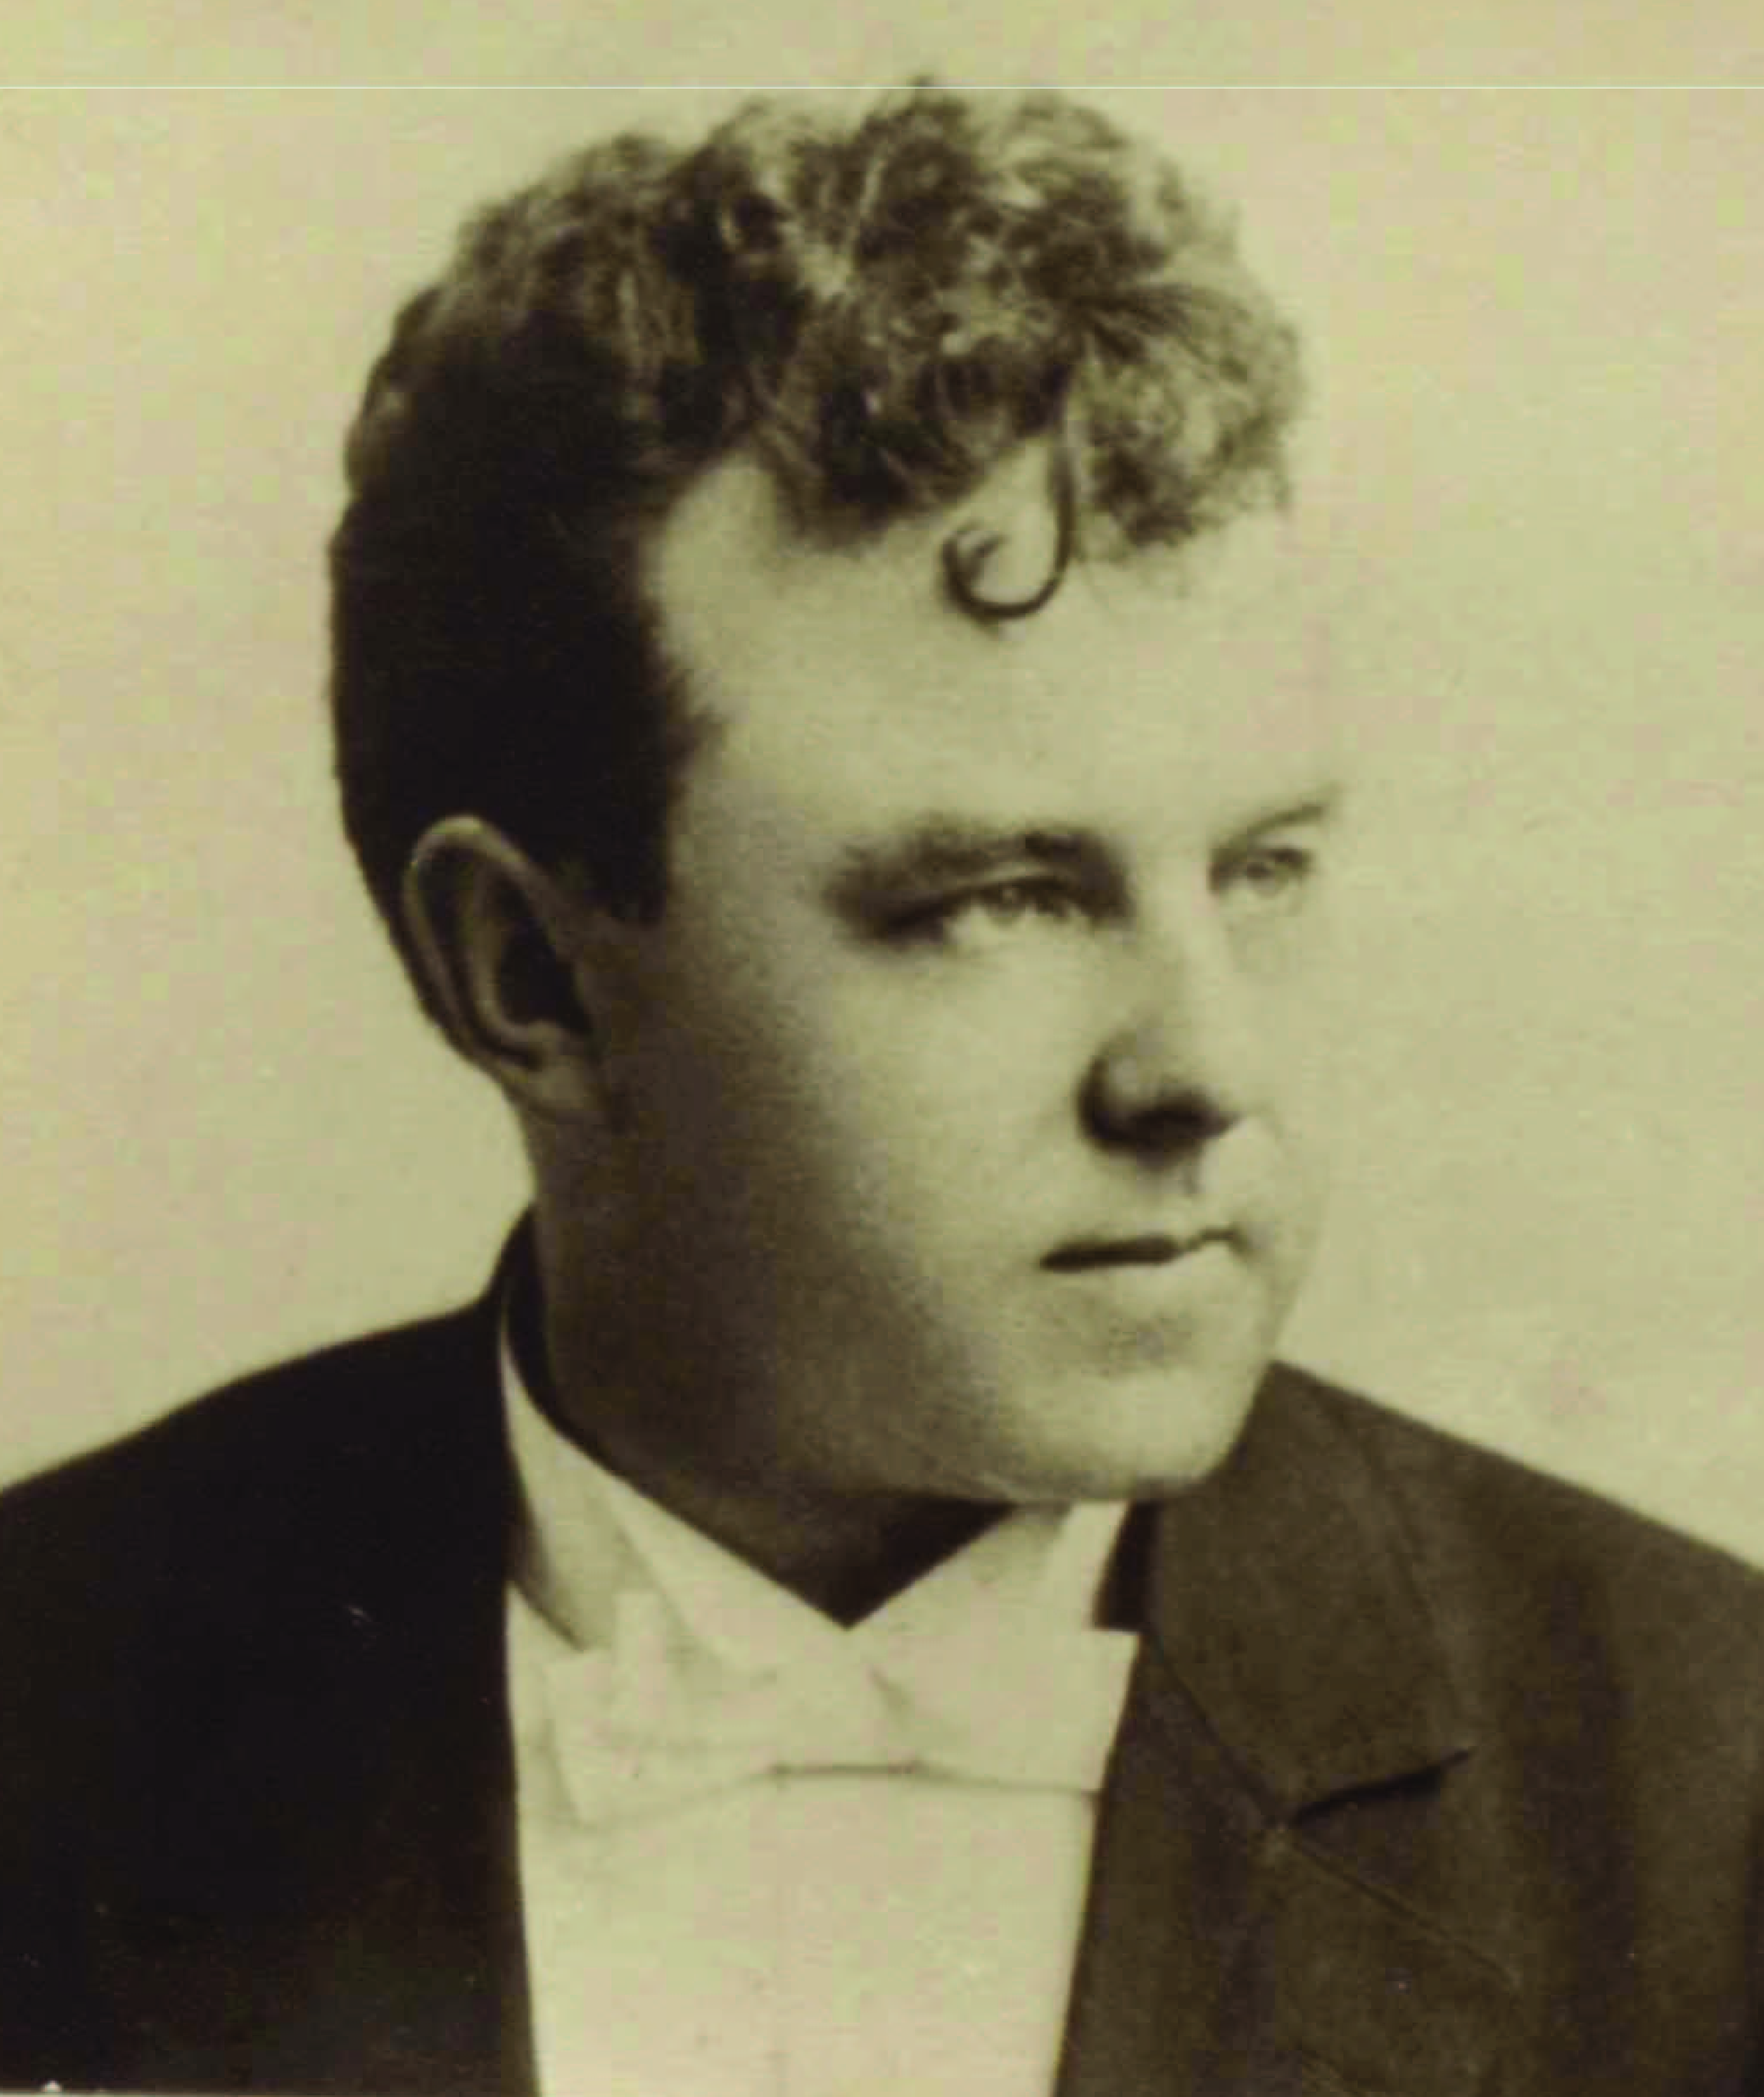
\includegraphics[width=\textwidth, height=\textheight, keepaspectratio]{233-a-hanus_lasek}
\caption{Hanuš Lašek (1860 – 1937)}
\label{fig:233-a-hanus_lasek}
\end{figure}

             \begin{figure}
\centering
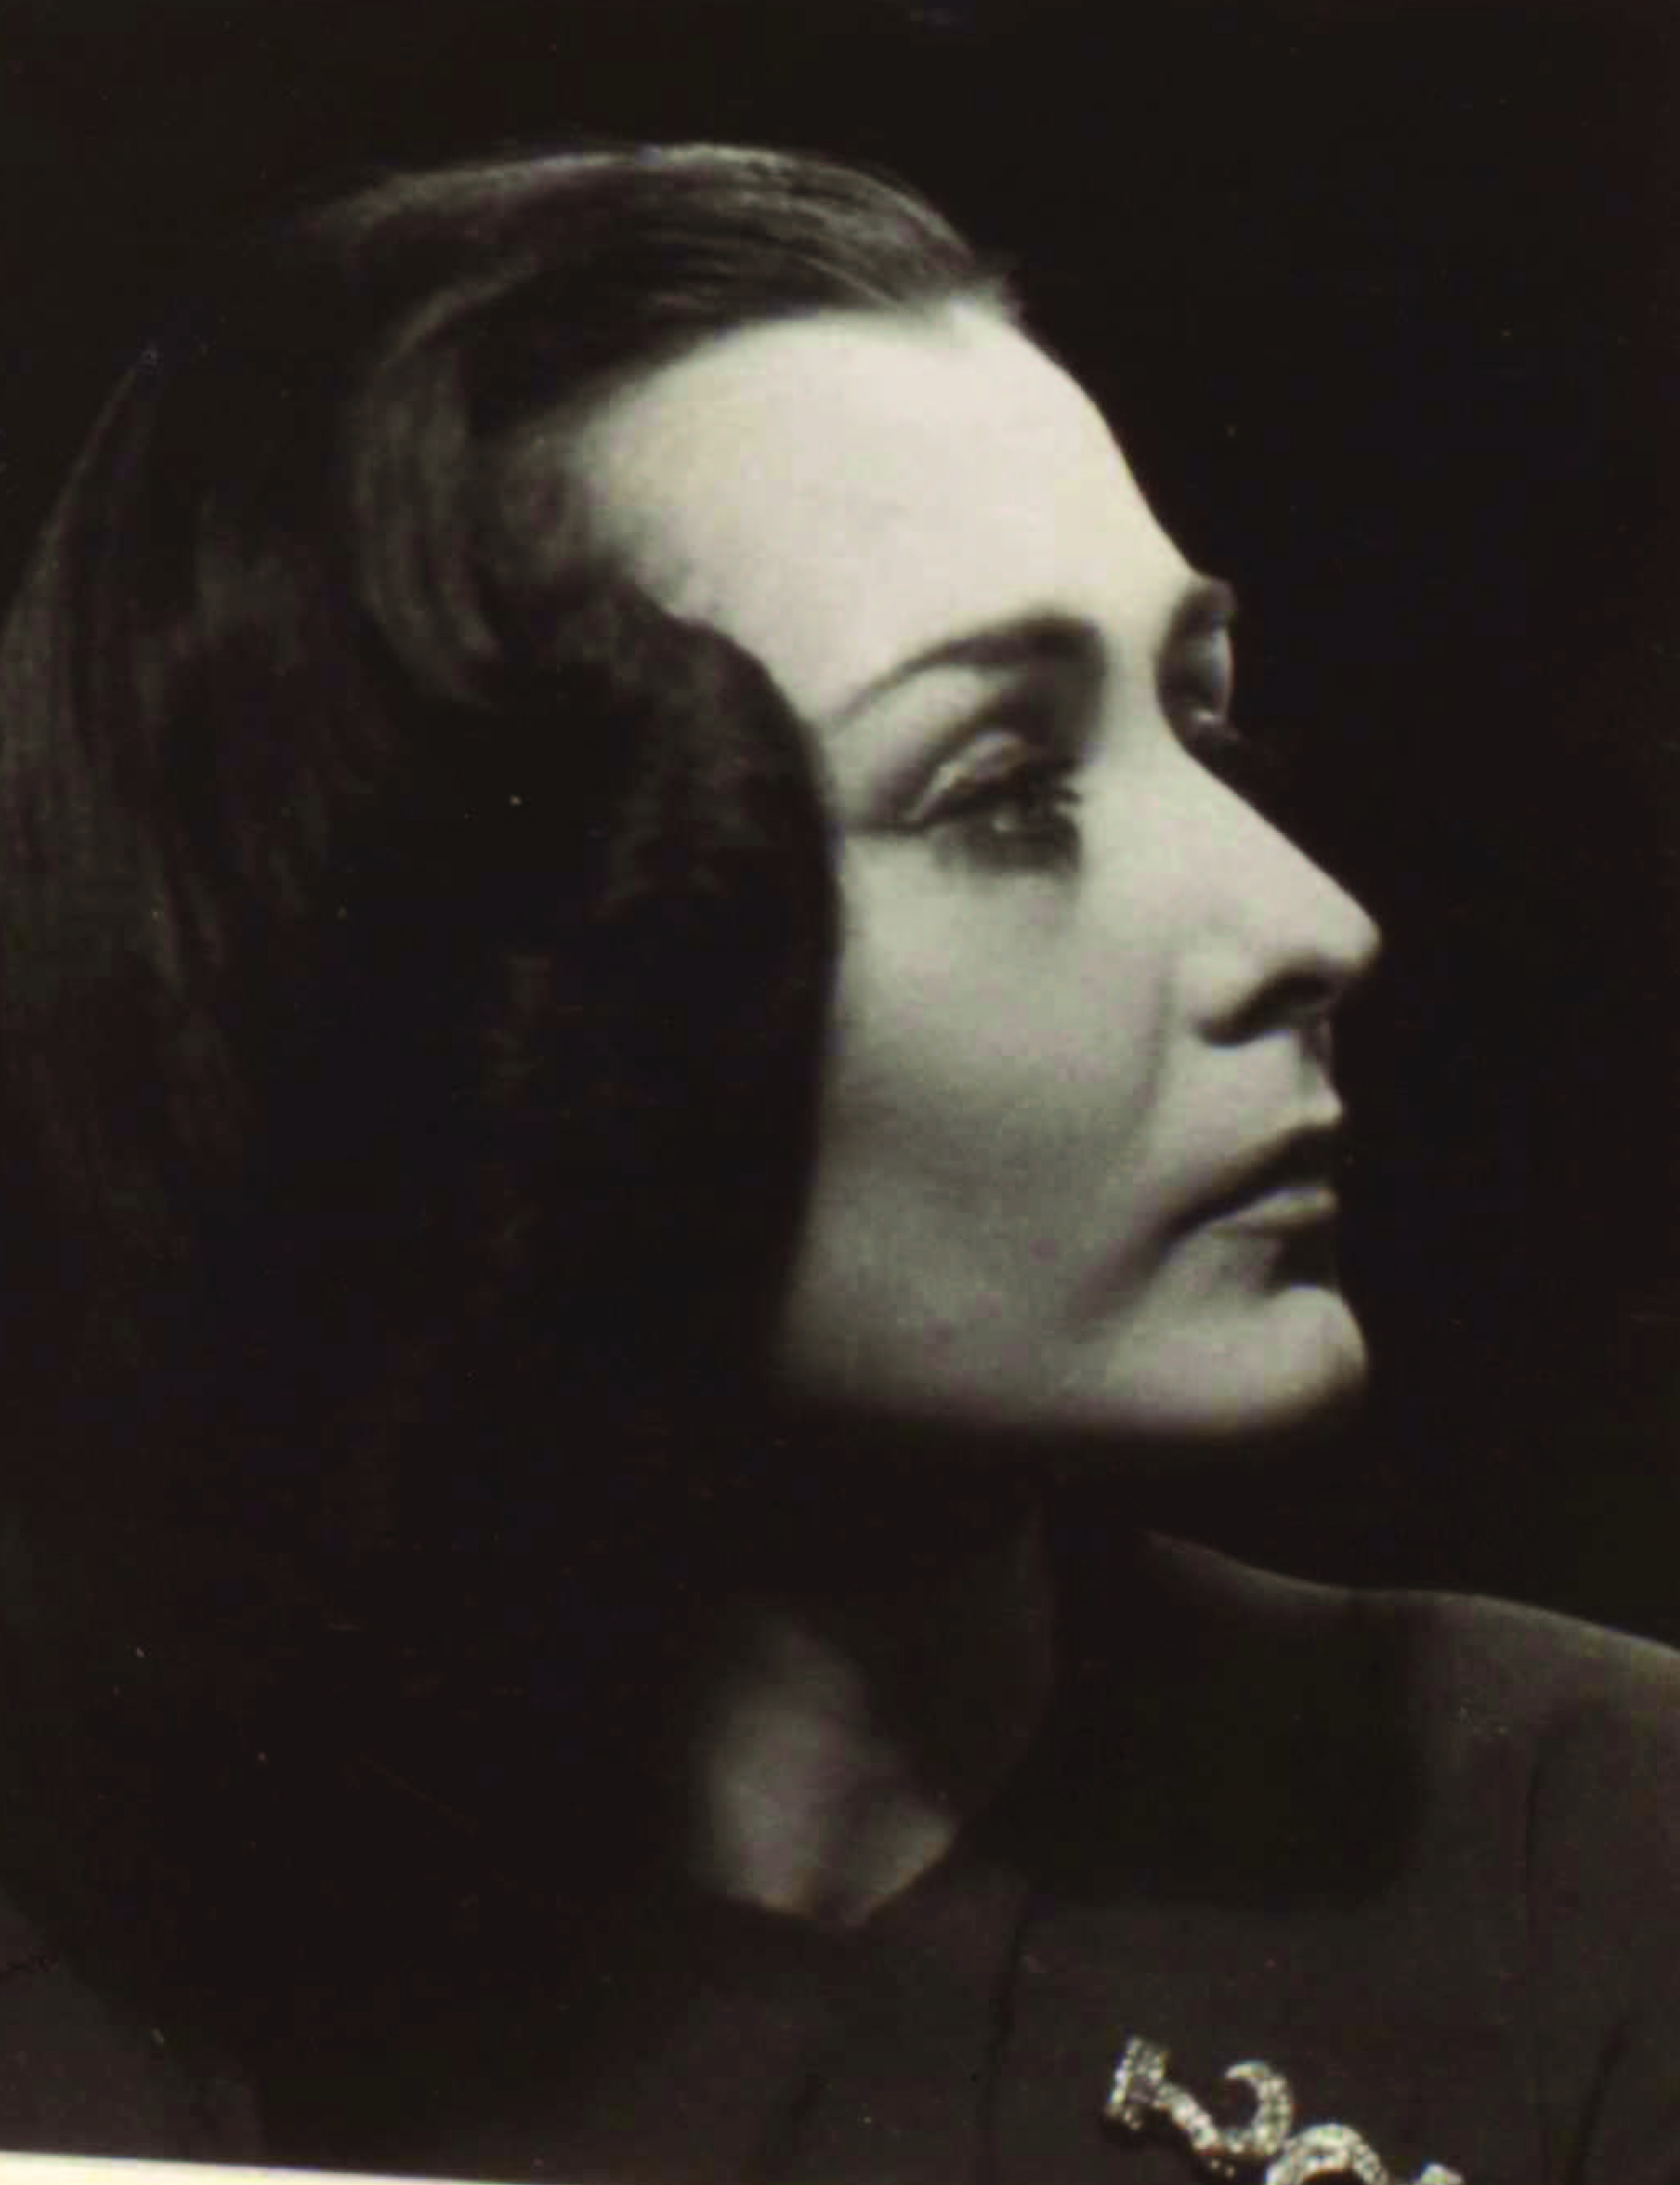
\includegraphics[width=\textwidth, height=\textheight, keepaspectratio]{233-b-hana_vitova_laskova}
\caption{Význačnými potomky Josefy Prusíkové, provdané Laškové v Plasích, byl její syn Hanuš Lašek, slavný operní pěvec a jeho dcera filmová herečka Hana Vítová-Lašková }
\label{fig:233-b-hana_vitova_laskova}
\end{figure}

\end{document}
